\section{The Heart of a Lion}

\begin{wrapfigure}{rt}{.3\textwidth}
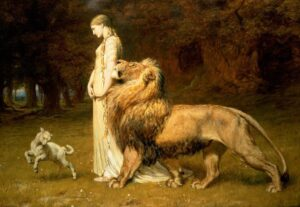
\includegraphics[width=.3\textwidth]{LionAndMaiden-300x207.jpg}
\end{wrapfigure}

Sometimes I feel like a lion wandering aimlessly across the savanna --- peeing on the bushes to stake out my territory, eating to satiation, gazing intently at the lionesses. The sun sets, the sun rises ... I have cheated death.

\paragraph{The Wisdom of a Knight Errant}


``You should know, Sancho,'' said Don Quixote, ``that love shows no restraint, and does not keep within the bounds of reason as it proceeds, and has the same character as death: it attacks the noble palaces of kings as well as the poor huts of shepherds, and when it takes full possession of a heart, the first thing it does is to take away fear and shame.''

Sancho: ``My master is valiant, intelligent, and in love.''

\paragraph{Facebook, forgetting and forgiving}


At the final Judgement, there is hope that the Most Merciful God will forgive our sins and blot them out of memory forever. Facebook neither forgives not forgets.

\paragraph{Everyone Hurts}


Recently, two athletes, who abandoned their commitments, have been praised for their courage. Each of them asserted that their ``mental health'' required it. I'd like to point out that everyone is hurting. How many people experience anxiety or depression, yet show up to work day after day. Athletes today are lionized for quitting and get more endorsements. Ordinary folk will lose their jobs.

\paragraph{Walking to First}


My Mother was very loving, but is only after some time has passed can I see how she guided me. She was tender when necessary but tough on me whenever I showed weakness. One morning I was tardy, so I had to walk to kindergarten alone. Terrified, I felt I was walking through a jungle. The streets, normally filled with the sound of children, were eerily silent. Every barking dog seemed like a threat. At that time, dogs roamed freely and there was one dog in particular that always chased me. I was in dread walking past his house. The final obstacle was the main drive whose traffic I needed to dodge. I made it to school and checked myself in. Suburban mothers will not do that today.

\paragraph{Perfect Grammar}


The Lone Ranger spoke grammatically correct English and there are few of us left. It sounds trivial, but it isn't. Michel de Montaigne :

\begin{quotex}
The greater part of the world's troubles are due to questions of grammar.
\end{quotex}


\paragraph{Thoughts on the Olympics}


\textbf{Archery}: The Huns could hit a moving target while riding on horseback with homemade bows and arrows. I would watch that for sure. But these archers with high tech bows and machine tooled arrows are boring. And they're probably all on beta blockers.

\textbf{Fencing}: I've watched enough movies, so I know that a good sword fight should take 10 minutes or so, and requires a lot of space. That would make compelling TV. These 10 second jousts don't seem real to me.

\textbf{Rowing}: A galley slave used to be the worst job in the world; now rowing is an Olympic sport.

\textbf{Equestrianism}: The equestrian horses are impressive with their dances. I wonder if, for his reward, the horse gets to party with geisha horses.

\textbf{Clothing}: For ``beach sports'', it is entirely appropriate to wear beach costumes, common to our age: bikinis for women and shorts for men. To counter an absurd objection, men do not wear Speedos to the beach. Nevertheless, they do were Speedos for swimming events and women wear costumes they help them glide. If women still want to sexualize men's sports, they should watch wrestling and weight lifting in which their entire sac is outlined.

\paragraph{Ibn Arabi's Dream}


Someone sent me this poem, right after I had had a similar dream. Now I understand it.

\begin{quotex}
I saw a girl in my sleep who did not, so far as I could see, and so far as my sight can judge, Have a sister equal to her in the beauty of her form --- a girl of Turkish race, whose light covered my gaze. 

I entered her in the vision, and she came towards me for me to gain my desire in embracing her.

Pleasure spread over my limbs, and on waking, I did not find any trace.

So I said, `Well-being and relief must surely come; God's determination will bring it, walking with the divine decree.'

I interpreted seeing her genitals (farj) as meaning that I would see relief (faraj), taking away from me the clothing of misery and harm.

For I have never seen a more perfect vision bringing joy to me like her before in my life.

I called it a sighting (ru'ya) and did not call it a dream (ru'yā), because of the danger that dreams bring.
\end{quotex}


\paragraph{The Possible and the Real}


Tradition teaches about the possible and the real. With larger population, more possibilities can manifest. That is why we are experiencing change at such a vertiginous pace.

\paragraph{Give them what they want}


To be popular, it is advisable to give people what they want, not what they need. Usually, that involves sentimentalism. Frithjof Schuon tells this story about Abd al-Qadir al-Jilani:

\begin{quotex}
The saint relates a story about cats and the whole audience begins to weep from spiritual emotion.

They listened with boredom to the brilliant sermon of the great theologian.
\end{quotex}


\paragraph{The Myth of Er}


JE claimed: ``I have always subscribed to the traditional doctrine that we have wished all relevant events in our life before birth.'' That is just a restatement of the Myth of Er from Plato's \emph{Republic}.

Even Adam was give the choice. At first he was reluctant to be born into a body made of clay, but relented when he heard the celestial music.

\paragraph{Ace in the Hole}


``It's been a nice day, Chuck, I feel like smiling.''

But it wasn't nice for others. 

\emph{Ace in the Hole}\footnote{\url{https://www.imdb.com/title/tt0043338/mediaindex/?ref\_=tt\_mv\_sm}} is a 1951 classic film that illustrates the unholy alliance of amoral journalists and corrupt politicians. The media and corrupt politicians conspire to create a ``story'' out of a random event. They extend the event beyond what is necessary to resolve it, just to milk it. With a well-crafted narrative, the public is emotionally manipulated and drawn in. A ``victim'' is identified and nearly eulogized. Other characters are also media creations, barely resembling their real-life counterparts.

Leo gets trapped in a cave while collecting Indian artifacts. Chuck is the journalist who sees the story as an opportunity for a ``big story''. Instead of going straight in to rescue Leo, Chuck convinces the local sheriff to drill from above, which will take several days. By promising to make the sheriff a national hero, Chuck bends events for his benefit. In the next few days, the mountain becomes a tourist attraction filled with people.

Lorraine despises her husband Leo, but Chuck describes them as a loving couple. We see Lorraine biting into an apple, with the obvious symbolism. She tries to seduce Chuck with the line above, with a seductive look worthy of the best of the undines. Ultimately, Leo dies due to Chuck's ambition.

Keep all this in mind if you ever waste your time with TV news or ``journalists''. The only difference is that in the movie, the bad guy gets his comeuppance.

\paragraph{Only from you my sweet Love}

\begin{verse}
Only from you, my sweet love,\\
Shall this heart find peace and solace\\
Your beautiful hazy eyes are the stars\\
By which love guides me to port.
\end{verse}

\url{https://www.youtube.com/watch?v=DgOcvWe60xI}

\flrightit{Posted on 2021-08-06 by Cologero}

